\documentclass[11pt]{article}
\usepackage[margin=1in]{geometry}
\usepackage[T1]{fontenc}
\usepackage[utf8]{inputenc}
\usepackage{lmodern,microtype,amsmath,amssymb,amsthm,mathtools}
\usepackage{booktabs,graphicx,enumitem,natbib,xcolor}
\usepackage[colorlinks=true,allcolors=blue!55!black]{hyperref}
\setlist{nosep}
\newtheorem{theorem}{Theorem}
\newtheorem{lemma}{Lemma}
\theoremstyle{remark}
\newtheorem{remark}{Remark}
\newcommand{\R}{\mathbb R}
\newcommand{\E}{\mathbb E}
\newcommand{\PP}{\mathbb P}
\newcommand{\ip}[2]{\langle #1,#2\rangle}
\newcommand{\norm}[1]{\lVert #1\rVert}
\newcommand{\rank}{\operatorname{rank}}
\newcommand{\soft}{\operatorname{soft}}
\newcommand{\TV}{\operatorname{TV}}
\newcommand{\Tu}{\mathrm{Tu}}
\newcommand{\TT}{\mathrm{TT}}
\newcommand{\NL}{\mathrm{NL}}
\newcommand{\calL}{\mathcal L}
\title{Joint Tensor Rank Constraints Can Shorten\newline Honest Functional Confidence Intervals}
\author{Research working draft}
\date{September 9, 2026}

\begin{document}
\maketitle
\begin{center}
\fbox{\begin{minipage}{0.91\textwidth}\small
\textbf{Status.} The six numbered theorems have complete derivations in the appendix and supplementary numerical checks. This is a working research note, without independent proof review or a claim of certified priority. Sharp minimax length, general loading geometry and adaptation to the actual rank remain open. No conjecture is stated as a theorem.
\end{minipage}}
\end{center}

\begin{abstract}
We study confidence intervals for a prescribed linear functional of a fully observed Gaussian tensor mean, under a known Frobenius bound and upper bounds on its Tucker or tensor-train ranks. Actual ranks may be smaller than the supplied caps, and nonzero singular values may be arbitrarily small. For an orthogonal tensor contrast, canonical decompositions imply an $\ell_{2/K}$ bound on the relevant diagonal, where $K$ is the tensor order. Classical soft thresholding then gives an explicit finite-sample honest interval. For equal mode size $p$, fixed rank caps, normalized diagonal loading and norm bound $M=\tau\sqrt p$, its length is $O\{\tau(\log p/p)^{(K-2)/(2K)}\}$, where $\tau$ is the coordinate noise standard deviation. When $K\ge3$, this is smaller in order than every fixed-radius affine interval on the same class, and than the expected length at zero of every interval required to cover the larger class defined by one unfolding constraint. A within-class lower bound leaves a polynomial minimax gap. In 172 Gaussian configurations with 2,000 replications each, the selected interval has empirical coverage between 99.75\% and 100\%, indicating substantial conservatism. The results establish two specific length comparisons; they do not establish unrestricted optimality or adaptation to the actual rank.
\end{abstract}

\noindent\textbf{Keywords:} honest confidence intervals; linear functionals; Gaussian sequence model; tensor train; Tucker rank; nonconvex parameter space.

\section{Introduction}\label{sec:intro}

Low-rank tensor models impose several rank restrictions simultaneously. Whether these restrictions help estimation is different from whether they permit shorter confidence intervals that remain valid when components vanish. Consider a third-order $p\times p\times p$ tensor mean $A$, observed through $n=p$ independent full tensors with independent standard Gaussian errors. Its sample mean has coordinate noise level $\tau=p^{-1/2}$. Suppose $\norm A_F\le1$ and the tensor has rank at most one. Our running estimand is the normalized diagonal sum $p^{-1/2}\sum_{i=1}^p A_{iii}$. The direct Gaussian interval is valid regardless of rank. The question is whether the tensor restriction permits a substantially shorter interval while retaining coverage at every admissible signal, including zero.

Several parts of this question have established precedents. Tensor functional inference on regular low-rank strata is developed by \citet{xu2025}; matrix inference without estimating the exact rank is available under quantitative conditions \citep{choi2026}. Honest adaptation and nonlinear functional estimation on nonconvex classes have a much older theory \citep{cailow2004,cailownonconvex2004}. Consequently, neither unknown rank nor nonlinear inference is a sufficient novelty claim. A more specific question is whether the simultaneous tensor restrictions produce an inferential advantage that disappears when the honesty class retains only one unfolding rank constraint.

We answer this restricted comparison for a class of prescribed orthogonal loadings. The observation model is a Gaussian location experiment with known noise variance, and the norm and rank caps are supplied. We require finite-sample coverage over the entire cap class, with no lower bound on any nonzero singular value. For fixed order $K\ge3$, equal mode size $p$ and $M=\tau\sqrt p$, we construct an interval of length $o(\tau)$. We then show that an honest fixed-radius affine interval on the same class must have length of order at least $\tau$, and that every interval honest over a single-unfolding relaxation must have expected length of order at least $\tau$ at zero. Matricization itself preserves all the data; the comparison concerns enlarging the parameter space.

Three issues govern the argument. First, a bound valid at rank boundaries must avoid inversion of small singular values. Second, a comparison with the relaxed model must cover all interval procedures on that model, rather than one chosen estimator. Third, a constructive upper bound must be distinguished from a sharp minimax result. The last distinction matters here: the lower bound inside the joint tensor class does not match the thresholding upper bound.

Canonical Tucker and tensor-train expansions provide a controlled sum of squared component weights. Applied to an orthogonal diagonal, this yields an $\ell_{2/K}$ envelope. The exponent is familiar from tensor factor quasi-norm geometry \citep{fan2023}; the estimator uses classical thresholding \citep{donohojohnstone1994}. A simultaneous Gaussian noise bound converts that envelope into an honest scalar interval. Gaussian mixtures with a common functional value supply the relaxed-class and within-class lower bounds. In the running third-order example, the resulting radius is at most $\tau\{8\log(2p/\alpha)/p\}^{1/6}$, despite the absence of an identifiable nonzero factor at the origin.

The note makes three concrete contributions to this restricted formulation:
\begin{enumerate}
\item An explicit diagonal bound for Tucker and TT cap classes, and a finite-sample interval valid across their lower-rank strata (Sections~\ref{sec:method}--\ref{sec:theory}).
\item Two quantitative separations: from fixed-radius affine intervals under the same honesty class, and from all intervals under a one-unfolding relaxation (Section~\ref{sec:theory}).
\item A within-class lower bracket and reproducible experiments that expose the remaining lack of sharpness and actual-rank adaptation (Sections~\ref{sec:gap}--\ref{sec:sim}).
\end{enumerate}
The precise separation appears distinct from the inspected literature, but its elementary ingredients make a reduction to existing general theory a serious remaining novelty question.

\section{Related work}\label{sec:related}

\paragraph{Functional inference and nonconvex classes.}
Optimal recovery connects confidence and estimation problems to parameter-set geometry \citep{donoho1994}. Nonlinear improvements on nonconvex classes and the limits of honest adaptation are established themes \citep{cailownonconvex2004,cailow2004,low1997}. Finite unions of convex classes admit general aggregation and functional-inference constructions \citep{juditskynemirovski2020}. These results supply both tools and a substantial novelty threat: the thresholding step below is not a new general inference principle. The particular comparison requires an upper bound exploiting joint tensor restrictions and a lower bound over the enlarged unfolding class.

\paragraph{Matrix and tensor uncertainty quantification.}
Low-rank matrix linear forms, geometric inverse problems and rank-cap confidence sets already have extensive theory \citep{xiayuan2021,cailiangrakhlin2016,carpentierkim2018,carpentieretal2018}. Tensor inference includes subspace and functional results in strong-signal regimes \citep{xiazhangzhou2022,agterberg2024}, as well as uncertainty quantification for tensor completion \citep{caipoorchen2023}. Our fully observed experiment is simpler than completion or random-design regression. Our loading is also narrower than an arbitrary functional. What changes is the uniformity class: every tensor below the supplied caps is covered, without a minimum-signal condition. The resulting interval is not asserted to retain regular-stratum efficiency.

\paragraph{Weak factors and singularity.}
Weak-factor inference, rank uncertainty and adaptation obstructions are studied in econometrics \citep{zhu2019,armstrong2026,choi2026}; uniform inference near critical matrix signal strengths is also under active development \citep{bykhovskaya2025}. Singular likelihood asymptotics \citep{drton2009} and universal inference \citep{wasserman2020} further show why validity at a singularity is not itself a new objective. Here the target is a tensor contrast, and the claim is a specific length separation.

\paragraph{Tensor geometry.}
Orthonormal Tucker representations and TT canonicalization are standard \citep{delathauwer2000,oseledets2011}. Tensor norm geometry and factor penalties are developed by \citet{friedlandlim2018,fan2023}, while rank-variety tangent cones are studied by \citet{gao2025,kutschan2018}. Our proof uses canonical expansions rather than estimating tangent spaces. The explicit rank constants below are sufficient bounds; their optimality is unknown. A companion literature dossier records 20 closest competitors, theorem assumptions and source-inspection depth, with a bibliography covering relevant work available by September 9, 2026.

\section{Experiment and parameter classes}\label{sec:model}

Let $K\ge2$, $p_k\ge1$, and $D=\prod_{k=1}^K p_k$. We observe
\begin{equation}\label{eq:model}
 Z=A+\tau G\in\R^{p_1\times\cdots\times p_K},\qquad
 \operatorname{vec}(G)\sim N(0,I_D),\qquad \tau>0.
\end{equation}
The noise level is known. Equivalently, $Z$ is the sufficient sample mean of independent full observations $W_j=A+\sigma G_j$, $j=1,\ldots,n$, with known $\sigma$ and $\tau=\sigma/\sqrt n$. This is an exact Gaussian mean equivalence, not an equivalence to scalar-response tensor regression. The observed variables are the tensors $W_j$, or $Z$; $A$ is a fixed unknown parameter. Factor and core representations are nonunique coordinates, not additional latent random variables.

Write $A_{(k)}$ for the mode-$k$ unfolding and $A_{\langle k\rangle}$ for the matrix joining modes $1,\ldots,k$ against $k+1,\ldots,K$. For supplied positive integer caps, define
\begin{align}
 \Theta_{\Tu}(M,\bar r)&=\{A:\norm A_F\le M,\ \rank(A_{(k)})\le\bar r_k,\ k=1,\ldots,K\},\label{eq:tucker}\\
 \Theta_{\TT}(M,\bar r)&=\{A:\norm A_F\le M,\ \rank(A_{\langle k\rangle})\le\bar r_k,\ k=1,\ldots,K-1\}.\label{eq:tt}
\end{align}
The known bound $M$ is positive. Actual ranks may be smaller, including zero; nonzero singular values may be arbitrarily small. No incoherence or coordinate sparsity condition is imposed. Noise contamination, unknown covariance, missing observations and model misspecification are outside these parameterized experiments.

The prescribed loading has the form
\begin{equation}\label{eq:loading}
 L=\sum_{i=1}^m w_i V_i,\qquad
 V_i=\bigotimes_{k=1}^K v_{ki},\qquad
 v_{ki}^\top v_{kj}=\mathbf1\{i=j\},\qquad \norm w_2=1.
\end{equation}
Here $m\le\min_k p_k$, and each loading family is supplied independently of the data. Thus $\norm L_F=1$. Although this is restrictive, $L$ need not be sparse in the observation basis: known orthogonal mode rotations can make it dense. The estimand and relevant observations are
\begin{equation}\label{eq:diagonal}
 \psi(A)=\ip LA=\sum_iw_i a_i,\qquad
 a_i=\ip A{V_i},\qquad d_i=\ip Z{V_i}=a_i+\tau g_i,
\end{equation}
where the $g_i$ are independent standard normals.

An interval $C(Z)$ is honest at level $1-\alpha$ on $\Theta$ if
\begin{equation}\label{eq:honesty}
 \inf_{A\in\Theta}\PP_A\{\psi(A)\in C(Z)\}\ge1-\alpha.
\end{equation}
This is a finite-sample requirement, not a pointwise limit along a fixed-rank stratum. Length and expected length are the primary criteria. For example,
\begin{equation}\label{eq:minimaxcriteria}
 \calL_0(\Theta)=\inf_{C:\,\eqref{eq:honesty}}\E_0|C|,
 \qquad \calL_{\max}(\Theta)=\inf_{C:\,\eqref{eq:honesty}}\sup_{A\in\Theta}\E_A|C|.
\end{equation}
The infima range over all measurable intervals, allowing independent randomization. The usual squared Frobenius estimation loss has population risk $R_A(B)=\norm{B-A}_F^2+D\sigma^2$ and empirical risk $R_n(B)=n^{-1}\sum_j\norm{W_j-B}_F^2$. We do not minimize these risks or require a full-tensor estimator.

The principal asymptotic comparison in experiment~\eqref{eq:model} uses $p_k=m=p$, fixed $K\ge3$, fixed rank caps, and $M=\tau\sqrt p$. A concrete sequence is $M=\sigma=1$, $n=p$, so $D=n^K$. All finite-sample results below also apply away from that sequence.

\section{Interval construction}\label{sec:method}

Define
\begin{equation}\label{eq:constants}
 q=\frac2K,\quad
 J_{\Tu}=\min_k\prod_{\ell\ne k}\bar r_\ell,\quad
 J_{\TT}=\prod_{k=1}^{K-1}\bar r_k,\quad B=J^{1-q/2}M^q,
\end{equation}
where $J$ is chosen for the applicable class. Set
\begin{equation}\label{eq:threshold}
 \lambda=\tau\sqrt{2\log(2m/\alpha)},\qquad
 \widehat\psi_{\NL}=\sum_iw_i\soft_\lambda(d_i),\qquad
 \soft_\lambda(x)=\operatorname{sign}(x)(|x|-\lambda)_+.
\end{equation}
The three candidate intervals have radii
\begin{align}
 h_{\NL}&=\norm w_\infty B(2\lambda)^{1-q},&
 I_{\NL}&=[\widehat\psi_{\NL}-h_{\NL},\widehat\psi_{\NL}+h_{\NL}],\label{eq:nl}\\
 h_G&=z_{1-\alpha/2}\tau,&
 I_G&=[\ip LZ-h_G,\ip LZ+h_G],\label{eq:direct}\\
 h_0&=M\left(\sum_{i=1}^s w_{(i)}^2\right)^{1/2},&
 I_0&=[-h_0,h_0],\label{eq:zero}
\end{align}
where $|w_{(1)}|\ge\cdots\ge|w_{(m)}|$ and $s$ is the smaller of $m$ and the smallest supplied rank cap. Choose
\begin{equation}\label{eq:select}
 C_*=I_{j_*},\qquad j_*\in\arg\min_{j\in\{\NL,G,0\}}h_j,
\end{equation}
with a fixed rule for ties. This choice depends only on known quantities. Choosing an interval after examining its center or an estimated rank is a different procedure and is not justified by the proof.

The constants in \eqref{eq:constants} calibrate the threshold procedure~\eqref{eq:threshold}; the direct alternative~\eqref{eq:direct} supplies a valid fallback. Only $m$ contractions are used. For coordinate loadings, computation reads $m$ tensor entries and takes $O(m)$ operations. Obtaining contractions for a dense rotated loading has additional cost, which can be large. The procedure does not estimate a Tucker core, TT cores, factors or actual ranks.

\section{Statistical theory}\label{sec:theory}

All six numbered results have complete proofs in the appendix; the project ledger labels them \textbf{PROVED}. The label denotes the supplied derivation, not independent peer review. The results use the experiment and classes of Section~\ref{sec:model}. Lower-bound constants are stated for $0<\alpha<1/4$ when this simplifies positivity.

\subsection{Diagonal geometry and honest coverage}

\begin{theorem}[Orthogonal diagonal compressibility]\label{thm:diagonal}
For either class in \eqref{eq:tucker}--\eqref{eq:tt}, under loading \eqref{eq:loading},
\begin{equation}\label{eq:compress}
 \sum_{i=1}^m|\ip A{V_i}|^{2/K}\le J^{1-1/K}M^{2/K}.
\end{equation}
No minimum singular value is required.
\end{theorem}

The proof expands a canonical tensor representation into at most $J$ product terms whose squared component weights sum to $\norm A_F^2$. For TT tensors, these terms need not be orthogonal. A prefix-weight identity establishes the sum exactly; assuming termwise orthogonality would be an incorrect shortcut. H\"older's inequality and Bessel's inequality then give \eqref{eq:compress}. The rank factor may be loose, particularly for growing caps.

For rank cap one the diagonal image is exactly the ball $\{a:\sum_i|a_i|^{2/K}\le M^{2/K}\}$, as shown in Lemma~\ref{lem:image}. Thus the diagonal-only statistical experiment is precisely a classical Gaussian sequence problem on an $\ell_q$ ball. The full tensor experiment contains additional off-diagonal information. This reduction limits the novelty of the method and identifies where a stronger result would need to go beyond it.

\begin{theorem}[Finite-sample honest interval]\label{thm:coverage}
For every $0<\alpha<1$, each interval in \eqref{eq:nl}--\eqref{eq:zero} is honest on the applicable cap class. Consequently, $C_*$ is honest and has deterministic length
\begin{equation}\label{eq:length}
 |C_*|=2\min\{h_{\NL},h_G,h_0\}.
\end{equation}
\end{theorem}

The event $\max_i|\tau g_i|\le\lambda$ has probability at least $1-\alpha$. On this event soft thresholding satisfies
\[
 |\soft_\lambda(a_i+\tau g_i)-a_i|\le\min(|a_i|,2\lambda)
 \le |a_i|^q(2\lambda)^{1-q}.
\]
Summing proves the nonlinear interval bound. No central limit theorem, rank recovery or pilot remainder is needed. This simplicity also limits the contribution: once the diagonal envelope is known, the coverage argument is classical. Known $M$ is essential to the stated calibration.

\subsection{Two lower-bound comparisons}

For the remainder of this subsection let all dimensions equal $p$, let $E_i=e_i^{\otimes K}$, and put
\begin{equation}\label{eq:equalL}
 L=p^{-1/2}\sum_{i=1}^p E_i,\qquad z=z_{1-\alpha/2}.
\end{equation}

\begin{theorem}[Fixed-radius affine intervals]\label{thm:affine}
Suppose the honesty class contains $0$ and all $\pm M E_i$. If $0<\alpha<1/2$ and
\[
 C(Z)=[\ip WZ+b-h,\ip WZ+b+h]
\]
is honest, with deterministic $W,b,h$, then
\begin{equation}\label{eq:affinelower}
 h\ge\frac{(M/\sqrt p)z\tau}{M/\sqrt p+z\tau}.
\end{equation}
On the rank-one tensor Frobenius ball, the best radius in this affine class is therefore of order $\min(M/\sqrt p,\tau)$, up to constants depending on $\alpha$.
\end{theorem}

The theorem allows $W$ to use the entire tensor. It does not cover affine centers with data-dependent radii. The matching upper order follows by choosing between $I_G$ and $I_0$ for rank cap one.

For a nonempty proper subset $S$ of modes, write $A_{[S]}$ for the corresponding bipartition unfolding and define
\begin{equation}\label{eq:relax}
 \Theta_S=\{A:\rank(A_{[S]})\le1,\ \norm A_F\le M\}.
\end{equation}

\begin{theorem}[Cost of a single unfolding honesty class]\label{thm:unfolding}
If $0<\alpha<1/4$, every interval honest on $\Theta_S$ satisfies
\begin{equation}\label{eq:unfoldlower}
 \E_0|C|\ge c_\alpha\min\left\{\frac M{\sqrt p},\frac\tau4\right\},\qquad
 c_\alpha=1-2\alpha-\frac12\sqrt{\sqrt{8/7}-1}>0.
\end{equation}
The lower order $\min(M/\sqrt p,\tau)$ is attained up to $\alpha$-dependent constants by the direct/structural choice on $\Theta_S$.
\end{theorem}

The alternatives in the proof are rank one in the chosen matrix unfolding. They generally violate the other tensor rank constraints. This is necessary for the comparison: the theorem measures the cost of requiring coverage on the larger class. For Tucker caps, a mode unfolding is a permissible relaxation; for TT caps, a contiguous cut is permissible. With all tensor rank caps one, every bipartition in \eqref{eq:relax} contains the original tensor class. Increasing an unfolding cap further preserves the lower bound.

\begin{theorem}[Strict length separations]\label{thm:separation}
Let $K\ge3$ and the rank caps be fixed. Under \eqref{eq:equalL} and $M=\tau\sqrt p$, $C_*$ is honest on the Tucker or TT class and
\begin{equation}\label{eq:separation}
 |C_*|\le2\tau J^{1-1/K}
 \left\{\frac{8\log(2p/\alpha)}p\right\}^{(K-2)/(2K)}=o(\tau).
\end{equation}
In contrast, every fixed-radius affine interval honest on the same class has length at least $2z\tau/(1+z)$. Every interval honest on a class retaining only one constrained unfolding has expected length at zero at least $c_\alpha\tau/4$.
\end{theorem}

For growing caps, the same conclusion follows if $J^{1-1/K}(\log p/p)^{(K-2)/(2K)}\to0$. This condition may be restrictive. At $K=2$ the exponent in \eqref{eq:separation} is zero, so the argument gives no polynomial separation. Theorem~\ref{thm:separation} neither asserts that the displayed exponent is optimal nor compares favorably at every strong signal with an efficient oracle projection interval. Figure~\ref{fig:theory} displays the explicit comparisons and the within-class bracket established next.

\begin{figure}[t]
\centering
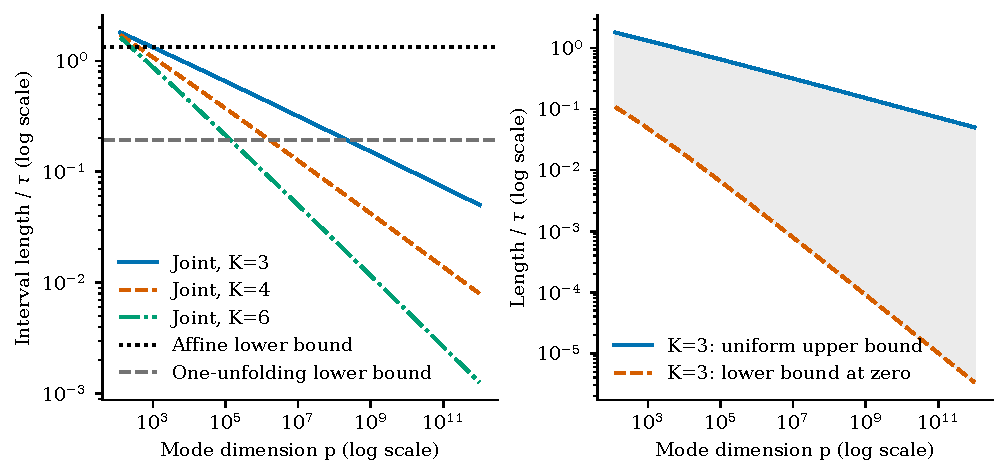
\includegraphics[width=\textwidth]{figures/theoretical_comparison.pdf}
\caption{Joint constraints permit a vanishing normalized length, while the within-class optimal rate remains unresolved. Left: analytic evaluations of the cap-one selected length and the affine and one-unfolding lower bounds, with $M=\tau\sqrt p$ and $\alpha=0.05$. Right: the proved upper and lower bounds for $K=3$; the shaded region is an unresolved bracket, not an uncertainty band. These are formulas evaluated up to $p=10^{12}$; Monte Carlo experiments stop at $p=8192$.}
\label{fig:theory}
\end{figure}

\subsection{What remains unknown inside the tensor class}\label{sec:gap}

\begin{theorem}[Within-class lower bound]\label{thm:jointlower}
For $0<\alpha<1/4$, every interval honest on a class containing the rank-one tensor Frobenius ball of radius $M$ satisfies
\begin{equation}\label{eq:jointlower}
 \E_0|C|\ge(3/4-2\alpha)
 \frac{\min\{M,\tau\sqrt{\log(1+p/4)}\}}{\sqrt p}.
\end{equation}
\end{theorem}

This is a sparse-coordinate mixture bound. At $M=\tau\sqrt p$, for fixed caps and fixed $K\ge3$, the results imply
\begin{equation}\label{eq:gap}
 c\tau\sqrt{\frac{\log p}p}
 \le\calL_0(\Theta)\le\calL_{\max}(\Theta)
 \le C\tau\left(\frac{\log p}p\right)^{(K-2)/(2K)}
\end{equation}
for sufficiently large $p$, with constants depending on $K$, the caps and $\alpha$. The ratio of the displayed scales grows as $(p/\log p)^{1/K}$. Thus \textbf{sharp minimax length is PARTIAL}, with both sides established but unmatched. A possible improvement using off-diagonal observations is \textbf{CONJECTURED}; no asserted result relies on it. In particular, the coordinate mixture is not proved least favorable, and the two criteria in \eqref{eq:minimaxcriteria} may differ.

\paragraph{Assumption audit.}
Gaussian isotropy gives the exact diagonal sequence and the likelihood-ratio identities. The threshold interval alone extends whenever a valid simultaneous coordinate noise envelope is supplied, but the direct alternative and lower bounds require their own calibration. Orthonormal loading families produce Bessel bounds and equal noise variances; arbitrary loadings are untreated. Canonical tensor expansions avoid a spectral gap but yield potentially large rank constants. Supplied caps and $M$ identify the outer honesty class; replacing them with unvalidated estimates is not covered. None of these assumptions should be described as a routine approximation for dependent LLM representations.

\section{Simulation study}\label{sec:sim}

\subsection{Protocol and baselines}
The simulation protocol was written after the theorem derivations and before implementation. It uses seed 20260909, 2,000 replications per configuration, and exact marginal observations of the diagonal coordinates needed by the procedures. Unused independent Gaussian coordinates of the full tensor need not be generated. This does not simulate a regression design or a tensor completion experiment.

The main grid takes $K\in\{2,3,4,6\}$, $p=n\in\{128,512,2048,8192\}$, $M=\sigma=1$, and rank cap one. Signals have the form $A=a u^{\otimes K}$, with $a\in\{0,0.02,0.2,1\}$ and $u$ uniform on a coordinate support. For nonzero signals, support sizes include one, $p$, and a value near $(a/\lambda)^{2/K}$, with duplicates removed. The latter places diagonal means near the threshold. Additional configurations vary $n/p$ and the valid threshold multiplier, and use cap two with a second component tending to zero. There are 175 configurations, of which three deliberately violate the iid Gaussian model.

We compare $I_G$, $I_0$, $I_{\NL}$ and $C_*$. For nonzero rank-one signals, a known-direction oracle is also included. If $U=u^{\otimes K}$ were supplied, then $c\ip UZ\pm z\tau|c|$, where $c=\ip LU$, is exact for $A=aU$. Its joint Gaussian noise with the diagonal is simulated exactly. This oracle has unavailable structural information and a smaller honesty class; it is not an implementation of an estimated-subspace method. Published strong-signal methods are compared through their assumptions rather than advertised as uniform baselines without a matching implementation.

Each output row reports coverage, binomial Monte Carlo standard error, an exact 95\% Clopper--Pearson interval, deterministic length, center bias and its standard error, and root mean squared center error. Width standard errors are zero because the radii are deterministic. Numerical proof checks separately examine 101,101 scalar soft-threshold cases, 120 random Tucker and 120 random TT tensors, and exact finite-binomial mixture second moments. They supplement rather than replace the proofs.

\subsection{Gaussian coverage and interval length}
Table~\ref{tab:coverage} summarizes the 172 in-model configurations. The selected interval is substantially conservative. Across configurations, direct Gaussian coverage ranges from 0.9365 to 0.9625, and selected coverage ranges from 0.9975 to 1. These extrema are descriptive, not simultaneous confidence limits for uniform coverage. At coverage 0.95, the Monte Carlo standard error with 2,000 replications is approximately 0.00487. When all replications cover, the exact binomial interval is approximately $[0.99816,1]$, despite a zero plug-in standard error.

\begin{table}[ht]
\centering
\begin{tabular}{lrrr}
\toprule
Method & Configurations & Min. coverage & Max. coverage \\
\midrule
Direct Gaussian & 172 & 0.9365 & 0.9625 \\
Structural & 172 & 1.0000 & 1.0000 \\
Threshold & 172 & 0.9975 & 1.0000 \\
Selected & 172 & 0.9975 & 1.0000 \\
Known-direction oracle & 117 & 0.9370 & 0.9615 \\
\bottomrule
\end{tabular}

\caption{Coverage extrema over the stated Gaussian configurations. The oracle is evaluated only for nonzero rank-one signals, giving fewer configurations and a different information set. Each configuration has 2,000 replications; configuration-level uncertainty is retained in the accompanying CSV.}
\label{tab:coverage}
\end{table}

At $p=n=8192$ and cap one, the selected lengths divided by $\tau$ are $2.0000$, $0.9622$, $0.6674$ and $0.4629$ for $K=2,3,4,6$, respectively. The direct length is $3.9199\tau$. These width values are exact evaluations of the formulas, not fitted empirical convergence rates. They agree with the order-dependent prediction, while the $K=2$ control shows no vanishing length ratio. A known-direction oracle can be much shorter for diffuse signals; there is no claim of pointwise oracle dominance.

\subsection{Weak rank and noise assumptions}
For the boundary experiment, set $K=3$ and cap two, and generate
\[
 A_\epsilon=\sqrt{1-\epsilon^2}\,U_1+\epsilon U_2,
 \qquad \epsilon\in\{0,0.001,0.01,0.1,0.5\},
\]
where $U_1,U_2$ are unit product tensors with disjoint mode supports. Each constrained unfolding has nonzero singular values $\sqrt{1-\epsilon^2}$ and $\epsilon$ for $\epsilon>0$; the actual rank becomes one at zero. Figure~\ref{fig:weak} shows coverage and length for concentrated supports at $p=8192$. The selected radius remains constant as $\epsilon$ vanishes. This demonstrates validity across the tested boundary and explicitly demonstrates the absence of actual-rank adaptation.

\begin{figure}[ht]
\centering
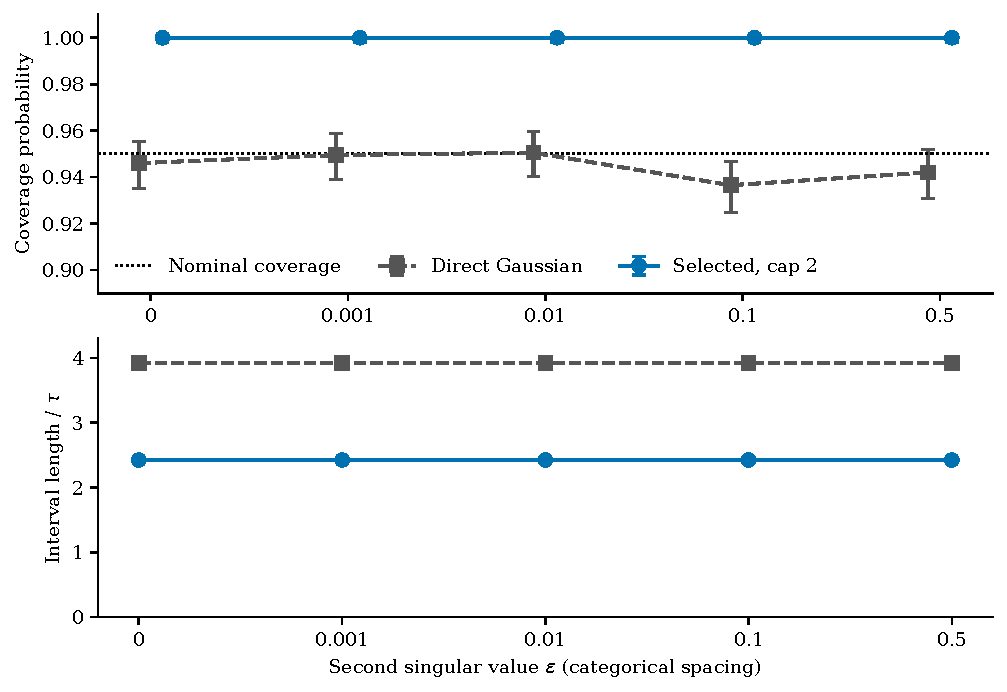
\includegraphics[width=\textwidth]{figures/weak_rank_coverage.pdf}
\caption{Coverage persists in the tested weak-component sequence, but the cap-based radius does not adapt to the actual rank. The setting is $K=3$, $p=n=8192$, $M=\sigma=1$ and cap two, with disjoint single-coordinate product factors. Top: empirical coverage and exact 95\% binomial intervals from 2,000 replications per value. Bottom: deterministic length divided by $\tau$. The horizontal spacing in $\epsilon$ is categorical.}
\label{fig:weak}
\end{figure}

Three additional zero-mean stress configurations use independent variance-one Student $t_3$ errors, a Gaussian mixture with 5\% of noise standard deviations multiplied by ten, and equicorrelated Gaussian coordinates with correlation 0.2. Table~\ref{tab:stress} reports the results. Variance contamination causes severe undercoverage for both procedures. Correlated Gaussian coordinates invalidate the direct iid variance but preserve the marginal Gaussian union bound used for the nonlinear interval. The Student result at zero is not a robustness theorem or evidence of coverage elsewhere.

\begin{table}[ht]
\centering
\begin{tabular}{lrr}
\toprule
Noise & Direct & Selected \\
\midrule
gaussian & 0.9540 & 1.0000 \\
student t3 & 0.9585 & 0.9670 \\
variance contamination & 0.5740 & 0.3830 \\
correlated & 0.1430 & 1.0000 \\
\bottomrule
\end{tabular}

\caption{Noise-assumption stress at $A=0$, $K=3$, $p=n=512$, cap one and nominal level 0.95. Only the first row belongs to the stated iid Gaussian model. These results delimit the calibration; they do not support a robustness claim.}
\label{tab:stress}
\end{table}

\section{Practical relevance and limits of an AI application}\label{sec:application}

The theory describes repeated, calibrated tensor measurements and a predetermined orthogonal contrast. A scientifically justified application would need a sampling model supporting the noise envelope, a credible outer norm/rank class, and a loading fixed independently of the observations. We do not supply a real-data experiment because no such dataset and calibration have been established in this project.

In particular, indexing an array by model, layer and prompt does not make iid Gaussian tensor location an adequate model for LLM representations. Repeated prompts, dependent tokens, layer coupling, heterogeneous measurement noise and data-selected contrasts materially change the experiment. An LLM example would currently add application terminology without additional statistical theory. A separate dependence and calibration analysis is required before such an experiment could substantiate this note.

\section{Discussion}\label{sec:discussion}

The central result is a concrete comparison of honesty classes. Under a special loading and bounded tensor ranks, a nonlinear interval can be smaller in order than every fixed-radius affine interval on the same class, and than every interval honest on a one-unfolding relaxation. The underlying tensor data need not be compressed or factor-estimated to obtain this comparison. Conversely, an algorithm using a matricized tensor can still exploit all original constraints; Theorem~\ref{thm:unfolding} does not rule out such an algorithm.

The current upper bound is not minimax sharp. The polynomial gap in \eqref{eq:gap} is the most important theoretical limitation, followed by the restricted loading, loose growing-rank constants, known norm and noise bounds, and lack of actual-rank adaptation. The experiments also show that the interval is conservative on the tested Gaussian grid. Strong-signal procedures or additional known-direction information may provide substantially better pointwise precision.

The most valuable next theorem would determine $\calL_0$ or $\calL_{\max}$ for the rank-one class, or characterize which loadings admit a joint-constraint advantage. A rank-adaptive procedure would additionally need honest calibration over the larger cap class and a theorem identifying the spectra or geometries on which shorter intervals are possible. A naive plug-in rank or variance estimate would not resolve these questions.

This draft is therefore a constructive research note and a basis for further theory, rather than a completed general solution to honest inference across unknown tensor ranks. The explicit separation was not found in the inspected literature, but the proof combines familiar ingredients. Its suitability for a strong statistics journal depends on resolving a substantial part of the remaining theory and confirming that the tensor specialization is not a direct consequence already established elsewhere.

\paragraph{Reproducibility.}
The accompanying project contains the prespecified simulation protocol, modular Python code, fixed seeds, 817 result rows, exact binomial uncertainty, source and result hashes, literature matrices, a theorem-status ledger and complete proof notes. All displayed numerical values are generated from the saved output or exact formulas. No real-data findings, robustness guarantees or conjectured rates are reported as established results.

\appendix
\section{Complete proofs}\label{app:proofs}

The proofs apply in finite dimensions. Constants used in the main text are explicit. All tensors and Gaussian variables are real.

\subsection{Canonical product expansions}

\begin{lemma}[Controlled squared component weights]\label{lem:cp}
For a tensor in either cap class there is a finite representation
\[
 A=\sum_{j=1}^{J_A}x_{1j}\otimes\cdots\otimes x_{Kj},\qquad
 a_j^{\mathrm{cp}}=\prod_{k=1}^K\norm{x_{kj}}_2,
\]
such that $J_A\le J$ and $\sum_j(a_j^{\mathrm{cp}})^2=\norm A_F^2$.
\end{lemma}

\begin{proof}
The zero tensor has a zero-term representation. For a nonzero Tucker tensor, choose orthonormal bases $U_k$ for the column spaces of its mode unfoldings. Orthogonal projection onto each such space leaves $A$ unchanged. Contracting these bases gives a core $\mathcal G$ with $A=\mathcal G\times_1U_1\cdots\times_KU_K$ and $\norm{\mathcal G}_F=\norm A_F$. The actual mode ranks satisfy $r_k\le\bar r_k$.

Fix a mode $k$. Expand all core indices other than $k$. Each tuple $j_{-k}$ gives unit factors $U_\ell[:,j_\ell]$ in modes $\ell\ne k$ and factor $U_k\mathcal G[:,j_{-k}]$ in mode $k$. Its squared product weight is $\norm{\mathcal G[:,j_{-k}]}_2^2$. These slice squares sum to $\norm{\mathcal G}_F^2$. The number of terms is $\prod_{\ell\ne k}r_\ell$. Choosing $k$ to minimize the corresponding cap product proves the Tucker assertion.

For a TT tensor, sequential matrix factorizations yield cores $G_k\in\R^{r_{k-1}\times p_k\times r_k}$, with $r_0=r_K=1$ and $r_k\le\bar r_k$. At each cut, factor the relevant matrix through a basis of its column space. Equivalently, left-orthogonalize the cores by QR and absorb the triangular factors into the next core. Thus the $(r_{k-1}p_k)\times r_k$ matrix associated with $G_k$ has orthonormal columns for $k<K$, and $\norm{G_K}_F=\norm A_F$. These steps use no inverse lower bound on a singular value.

Expand the contraction over all internal paths $(a_1,\ldots,a_{K-1})$. A path contributes the product tensor with physical vectors $G_k[a_{k-1},:,a_k]$. There are at most $\prod_{k<K}r_k\le J$ paths. To sum their squared weights, let
\[
 t_k(b)=\sum_{a_1,\ldots,a_{k-1}}
 \prod_{\ell=1}^k\norm{G_\ell[a_{\ell-1},:,a_\ell]}_2^2,
 \qquad a_k=b.
\]
Column normalization gives $t_1(b)=1$. If $t_{k-1}(a)=1$ for all $a$, then
\[
 t_k(b)=\sum_a t_{k-1}(a)\norm{G_k[a,:,b]}_2^2=1
\]
for $k<K$. Hence the sum of all squared path weights is
\[
 \sum_a t_{K-1}(a)\norm{G_K[a,:,1]}_2^2=\norm{G_K}_F^2=\norm A_F^2.
\]
The individual path terms need not be orthogonal; the prefix identity is what proves the required equality.
\end{proof}

\subsection{Proof of Theorem~\ref{thm:diagonal}}

\begin{proof}
Let $q=2/K\le1$ and use Lemma~\ref{lem:cp}. Subadditivity of the $q$th power of absolute value gives
\[
 \sum_i|\ip A{V_i}|^q
 \le\sum_j\sum_i\prod_{k=1}^K|\ip{x_{kj}}{v_{ki}}|^{2/K}.
\]
H\"older's inequality with $K$ equal exponents, followed by Bessel's inequality for each orthonormal family, yields
\begin{align*}
 \sum_i\prod_k|\ip{x_{kj}}{v_{ki}}|^{2/K}
 &\le\prod_k\left(\sum_i|\ip{x_{kj}}{v_{ki}}|^2\right)^{1/K}\\
 &\le\prod_k\norm{x_{kj}}_2^{2/K}=(a_j^{\mathrm{cp}})^q.
\end{align*}
Finally, the power-mean inequality (or H\"older with exponents $2/q$ and $2/(2-q)$) gives
\[
 \sum_j(a_j^{\mathrm{cp}})^q
 \le J_A^{1-q/2}\left\{\sum_j(a_j^{\mathrm{cp}})^2\right\}^{q/2}
 \le J^{1-q/2}M^q.
\]
This is \eqref{eq:compress}. For $J_A=0$ both sides of the first inequality are zero.
\end{proof}

\subsection{Exact rank-one diagonal image}

\begin{lemma}[Exact diagonal reduction]\label{lem:image}
Under \eqref{eq:loading}, the image of the rank-one tensor Frobenius ball of radius $M$ under $A\mapsto(\ip A{V_i})_{i=1}^m$ is exactly
\[
 \left\{a\in\R^m:\sum_i|a_i|^{2/K}\le M^{2/K}\right\}.
\]
\end{lemma}

\begin{proof}
One inclusion follows from Theorem~\ref{thm:diagonal} with $J=1$. Conversely, for any vector in the displayed ball, put
\[
 x_1=\sum_i\operatorname{sign}(a_i)|a_i|^{1/K}v_{1i},\qquad
 x_k=\sum_i|a_i|^{1/K}v_{ki},\quad k\ge2,
\]
and set $A=x_1\otimes\cdots\otimes x_K$. Orthonormality gives $\ip A{V_i}=a_i$ and
\[
 \norm A_F=\prod_k\norm{x_k}_2
 =\left(\sum_i|a_i|^{2/K}\right)^{K/2}\le M.
\]
The tensor has every Tucker and TT rank at most one. The zero vector is handled by the zero tensor.
\end{proof}

\subsection{Threshold error and structural radius}

\begin{lemma}[Scalar threshold envelope]\label{lem:soft}
If $|e|\le\lambda$ and $s=\soft_\lambda(x+e)$, then $s$ lies between zero and $x$ and
\[
 |s-x|\le\min(|x|,2\lambda).
\]
For $q\in(0,1]$, $t,u\ge0$, one also has $\min(t,u)\le t^q u^{1-q}$, with the continuous interpretation at zero.
\end{lemma}

\begin{proof}
For $x\ge0$, $x+e\ge-\lambda$, so thresholding cannot produce a negative value. Also $x+e-\lambda\le x$, so $0\le s\le x$. If $x>2\lambda$, then $x+e>\lambda$ and $x-s=\lambda-e\le2\lambda$. Otherwise $x-s\le x\le2\lambda$. The negative case follows by oddness. If $t\le u$, then $t=t^q t^{1-q}\le t^q u^{1-q}$; if $u\le t$, then $u=u^q u^{1-q}\le t^q u^{1-q}$.
\end{proof}

\begin{lemma}[Matrix functional bound]\label{lem:structural}
If $\rank(B)\le r$ and $H$ has singular values $s_1(H)\ge s_2(H)\ge\cdots$, then
\[
 |\ip HB|\le\norm B_F\left(\sum_{i\le r}s_i(H)^2\right)^{1/2}.
\]
\end{lemma}

\begin{proof}
Let $P$ project onto the column space of $B$. Then $PB=B$ and Cauchy--Schwarz gives $|\ip HB|=|\ip{PH}B|\le\norm{PH}_F\norm B_F$. Write $HH^\top=\sum_i\lambda_i u_i u_i^\top$, with decreasing nonnegative eigenvalues. The numbers $b_i=u_i^\top P u_i$ satisfy $0\le b_i\le1$ and $\sum_i b_i=\operatorname{tr}(P)\le r$. Therefore $\norm{PH}_F^2=\sum_i\lambda_i b_i\le\sum_{i\le r}\lambda_i$: moving any weight from a smaller eigenvalue to an unfilled larger one cannot reduce this sum. Since $\lambda_i=s_i(H)^2$, the result follows.
\end{proof}

\subsection{Proof of Theorem~\ref{thm:coverage}}

\begin{proof}
The product atoms are orthonormal because
\[
 \ip{V_i}{V_j}=\prod_k\ip{v_{ki}}{v_{kj}}=\mathbf1\{i=j\}.
\]
Gaussian isotropy then gives the independent normals in \eqref{eq:diagonal}. For a standard normal $g$, Chernoff's inequality gives $\PP(g>t)\le\exp(-t^2/2)$ by minimizing $\exp(-ut+u^2/2)$ at $u=t$. Apply the same inequality to $-g$ and take a union bound to obtain
\[
 \PP\{\max_i|\tau g_i|>\lambda\}
 \le2m\exp\{-\lambda^2/(2\tau^2)\}=\alpha.
\]
On the complementary event, Lemma~\ref{lem:soft} and Theorem~\ref{thm:diagonal} give
\begin{align*}
 |\widehat\psi_{\NL}-\psi(A)|
 &\le\norm w_\infty\sum_i\min(|a_i|,2\lambda)\\
 &\le\norm w_\infty(2\lambda)^{1-q}\sum_i|a_i|^q\le h_{\NL}.
\end{align*}
This proves the uniform coverage of $I_{\NL}$.

Because $\norm L_F=1$, $\ip LZ-\psi(A)\sim N(0,\tau^2)$, so $I_G$ has exact coverage. For any constrained unfolding, the loading matrix has singular values $|w_i|$: the product vectors on each side form orthonormal families. Lemma~\ref{lem:structural} thus gives $|\psi(A)|\le M(\sum_{i\le r}w_{(i)}^2)^{1/2}$. Choosing the smallest cap proves $|\psi(A)|\le h_0$, so $I_0$ has coverage one. The selected index in \eqref{eq:select} is deterministic, hence the selected interval retains its individual coverage without a multiple-selection correction. Its length is exactly \eqref{eq:length}.
\end{proof}

\subsection{Proof of Theorem~\ref{thm:affine}}

\begin{proof}
Set $t=\ip WL$. At $A=0$ the center error is normal with mean $b$ and standard deviation $v=\tau\norm W_F$. For fixed $h$ and $v>0$, the probability that this variable belongs to $[-h,h]$ is maximized at $b=0$. Indeed, for $b\ge0$ its derivative is
\[
 v^{-1}\{\phi((h+b)/v)-\phi((h-b)/v)\}\le0,
\]
since $|h+b|\ge|h-b|$; the function is even in $b$. Honesty at zero therefore implies $h\ge z\tau\norm W_F\ge z\tau|t|$. If $v=0$, the same last inequality is automatic.

At $A=\pm M E_i$, the mean center error is
\[
 b\pm M(\ip W{E_i}-p^{-1/2}).
\]
At least one sign has absolute mean at least $M|\ip W{E_i}-p^{-1/2}|$. A symmetric interval whose radius is strictly smaller than this mean magnitude has probability below $1/2$ under a nondegenerate normal distribution: it lies strictly to one side of the median. In the degenerate case the coverage is zero. Since $1-\alpha>1/2$, honesty forces
\[
 h\ge M\max_i|\ip W{E_i}-p^{-1/2}|
 \ge\frac M{\sqrt p}|1-t|.
\]
The last inequality follows from $t-1=p^{-1/2}\sum_i(\ip W{E_i}-p^{-1/2})$. Put $a=M/\sqrt p$ and $b'=z\tau$. The two bounds imply
\[
 1\le|1-t|+|t|\le h/a+h/b',
\]
which rearranges to \eqref{eq:affinelower}. On the rank-one tensor ball, $h_0=M/\sqrt p$, and the direct/structural choice gives the matching order. No result about arbitrary data-dependent widths is invoked.
\end{proof}

\subsection{A mixture inequality for confidence intervals}

\begin{lemma}[Common-target alternatives]\label{lem:mixture}
Let $P_0$ have target zero and let $Q$ be a mixture of alternatives whose targets all equal $\delta>0$. If $C$ covers zero under $P_0$ and covers the target at every alternative with probability at least $1-\alpha$, then
\begin{equation}\label{eq:mixtureCI}
 \E_0|C|\ge\delta\{1-2\alpha-\TV(P_0,Q)\}.
\end{equation}
If $Q\ll P_0$, then $\TV(P_0,Q)\le\frac12\sqrt{\chi^2(Q,P_0)}$.
\end{lemma}

\begin{proof}
Mixture coverage gives $Q(\delta\in C)\ge1-\alpha$. By the definition of total variation, $P_0(\delta\in C)\ge1-\alpha-\TV(P_0,Q)$. Intersecting with $\{0\in C\}$ gives probability at least $1-2\alpha-\TV$. An interval containing both points has length at least $\delta$, proving \eqref{eq:mixtureCI}. The divergence bound follows from Cauchy--Schwarz applied to $\frac12\E_0|dQ/dP_0-1|$. Appending an independent random seed leaves total variation unchanged, so randomized intervals are covered as well.
\end{proof}

For Gaussian shifts $P_B=N(\operatorname{vec}(B),\tau^2I_D)$, direct integration of their likelihood ratios gives
\begin{equation}\label{eq:LR}
 \E_0\left[\frac{dP_B}{dP_0}\frac{dP_C}{dP_0}\right]
 =\exp\{\ip BC/\tau^2\}.
\end{equation}
To verify this, each ratio is $\exp\{\ip ZB/\tau^2-\norm B_F^2/(2\tau^2)\}$. Multiply the ratios and use the moment generating function of $\ip Z{B+C}$, whose variance under $P_0$ is $\tau^2\norm{B+C}_F^2$. The exponent simplifies to \eqref{eq:LR}.

\subsection{Proof of Theorem~\ref{thm:unfolding}}

\begin{proof}
For the given bipartition, let $f_i=\bigotimes_{k\in S}e_i$ and $g_i=\bigotimes_{k\notin S}e_i$. Both families are orthonormal. Let $u=p^{-1/2}(s_1,\ldots,s_p)$ with independent uniform signs, and define
\[
 \theta=\min(M,\tau\sqrt p/4),\qquad
 A_u=\theta\left(\sum_i u_i f_i\right)\otimes
                    \left(\sum_j u_j g_j\right).
\]
Every alternative has rank one in this unfolding, norm $\theta$, and functional value $\delta=\theta/\sqrt p$. Let $Q$ average their Gaussian laws. If $v$ is an independent copy of $u$, then \eqref{eq:LR} gives
\[
 1+\chi^2(Q,P_0)=\E_{u,v}\exp\{\theta^2(u^\top v)^2/\tau^2\}
 =\E\exp\{a S_p^2/p\},
\]
where $S_p$ is a sum of $p$ independent signs and $a=\theta^2/(\tau^2p)\le1/16$.

Introduce an independent standard normal $H$. Its moment generating function yields
\begin{align*}
 \E\exp(aS_p^2/p)
 &=\E_H\left\{\cosh(\sqrt{2a/p}\,H)\right\}^p\\
 &\le\E_H\exp(aH^2)=(1-2a)^{-1/2}\le\sqrt{8/7}.
\end{align*}
The inequality uses $\log\cosh(x)\le x^2/2$: for $x\ge0$, its derivative $\tanh(x)$ is at most $x$, and both functions are even. The Gaussian-square expectation follows by integrating $\exp\{-(1-2a)h^2/2\}/\sqrt{2\pi}$; it is finite since $a<1/2$. Nonnegative integrands justify exchanging the expectations.

Lemma~\ref{lem:mixture} now gives \eqref{eq:unfoldlower}. The constant is positive for $\alpha<1/4$. On $\Theta_S$, Lemma~\ref{lem:structural} with loading singular values all equal to $p^{-1/2}$ gives $|\psi(A)|\le M/\sqrt p$. Choosing between this structural interval and the direct interval attains the lower order. All calculations use the entire Gaussian experiment; the result does not arise from hiding off-diagonal observations.
\end{proof}

\subsection{Proof of Theorem~\ref{thm:separation}}

\begin{proof}
Substitute $M=\tau\sqrt p$, $q=2/K$ and $\norm w_\infty=p^{-1/2}$ into \eqref{eq:nl}. This gives
\[
 h_{\NL}=\tau J^{1-1/K}
 p^{1/K-1/2}\{8\log(2p/\alpha)\}^{(K-2)/(2K)},
\]
which is the radius in \eqref{eq:separation}. For fixed $K\ge3$, its exponent $\beta=(K-2)/(2K)$ is positive and $(\log p/p)^\beta\to0$. The cap classes contain all $\pm M E_i$ and zero, so Theorem~\ref{thm:affine} gives radius at least $z\tau/(1+z)$. For any retained constrained unfolding, the corresponding matrix-rank cap class contains $\Theta_S$, and Theorem~\ref{thm:unfolding} gives expected length at zero at least $c_\alpha\tau/4$. The same comparisons under the stated growing-cap condition follow by retaining the factor $J^{1-1/K}$.
\end{proof}

\subsection{Proof of Theorem~\ref{thm:jointlower}}

\begin{proof}
Let $a=\min\{M,\tau\sqrt{\log(1+p/4)}\}$ and mix uniformly over $A_j=aE_j$, $j=1,\ldots,p$. Each is in the rank-one tensor class and has target $\delta=a/\sqrt p$. Orthogonality of the $E_j$ and \eqref{eq:LR} imply
\[
 1+\chi^2(Q,P_0)=p^{-2}\{p\exp(a^2/\tau^2)+p(p-1)\}.
\]
Thus $\chi^2(Q,P_0)=\{\exp(a^2/\tau^2)-1\}/p\le1/4$ and $\TV(P_0,Q)\le1/4$. Lemma~\ref{lem:mixture} gives \eqref{eq:jointlower}. This construction does not establish that these alternatives are least favorable.
\end{proof}

\section{Result status and unresolved claims}

Theorem~\ref{thm:diagonal} (diagonal envelope), Theorem~\ref{thm:coverage} (honest interval), Theorem~\ref{thm:affine} (affine radius), Theorem~\ref{thm:unfolding} (relaxed-class lower bound), Theorem~\ref{thm:separation} (two separations), and Theorem~\ref{thm:jointlower} (within-class lower bound) are labeled \textbf{PROVED} in the project ledger on the basis of these derivations. None asserts a previously unknown general inference principle.

Sharp minimax length and actual-rank/spectrum adaptation are \textbf{PARTIAL}: the current upper/lower bracket and valid cap-based procedure establish components but do not solve either target. The possibility of attaining the coordinate-mixture lower scale at zero using off-diagonal information is \textbf{CONJECTURED}; a more difficult mixture could invalidate that conjecture. General loadings, unknown norm/variance bounds, dependence, contamination and an LLM application require additional formulation and theory. They are not results of this manuscript.

\bibliographystyle{plainnat}
\bibliography{references}
\end{document}
